\subsubsection{L'utilisation d'un gestionnaire de versions: Subversion}

Nous avons choisi pour coordonner notre travail d'utiliser un gestionnaire de versions: Subversion, afin de pouvoir mieux voir les avancements de la programmation et pour pouvoir se coordonner plus facilement, et pour pouvoir mieux voir les changements. Subversion a été choisi préférentiellement à d'autres systèmes de gestion de version (tels git ou mercurial, qui sont plus performants) principalement pour sa simplicité, afin d'éviter un trop apprentissage de l'utilisation du gestionnaire de version, ce qui n'était pas l'objectif.

\subsubsection{La conception du diagramme de classes}
Nous avons choisi d'utiliser l'outil Dia afin de réaliser un diagramme des classes qui nous a permis de penser les différentes classes utilisées par le jeu et nous répartir le travail.

\begin{figure}[h]
\centering
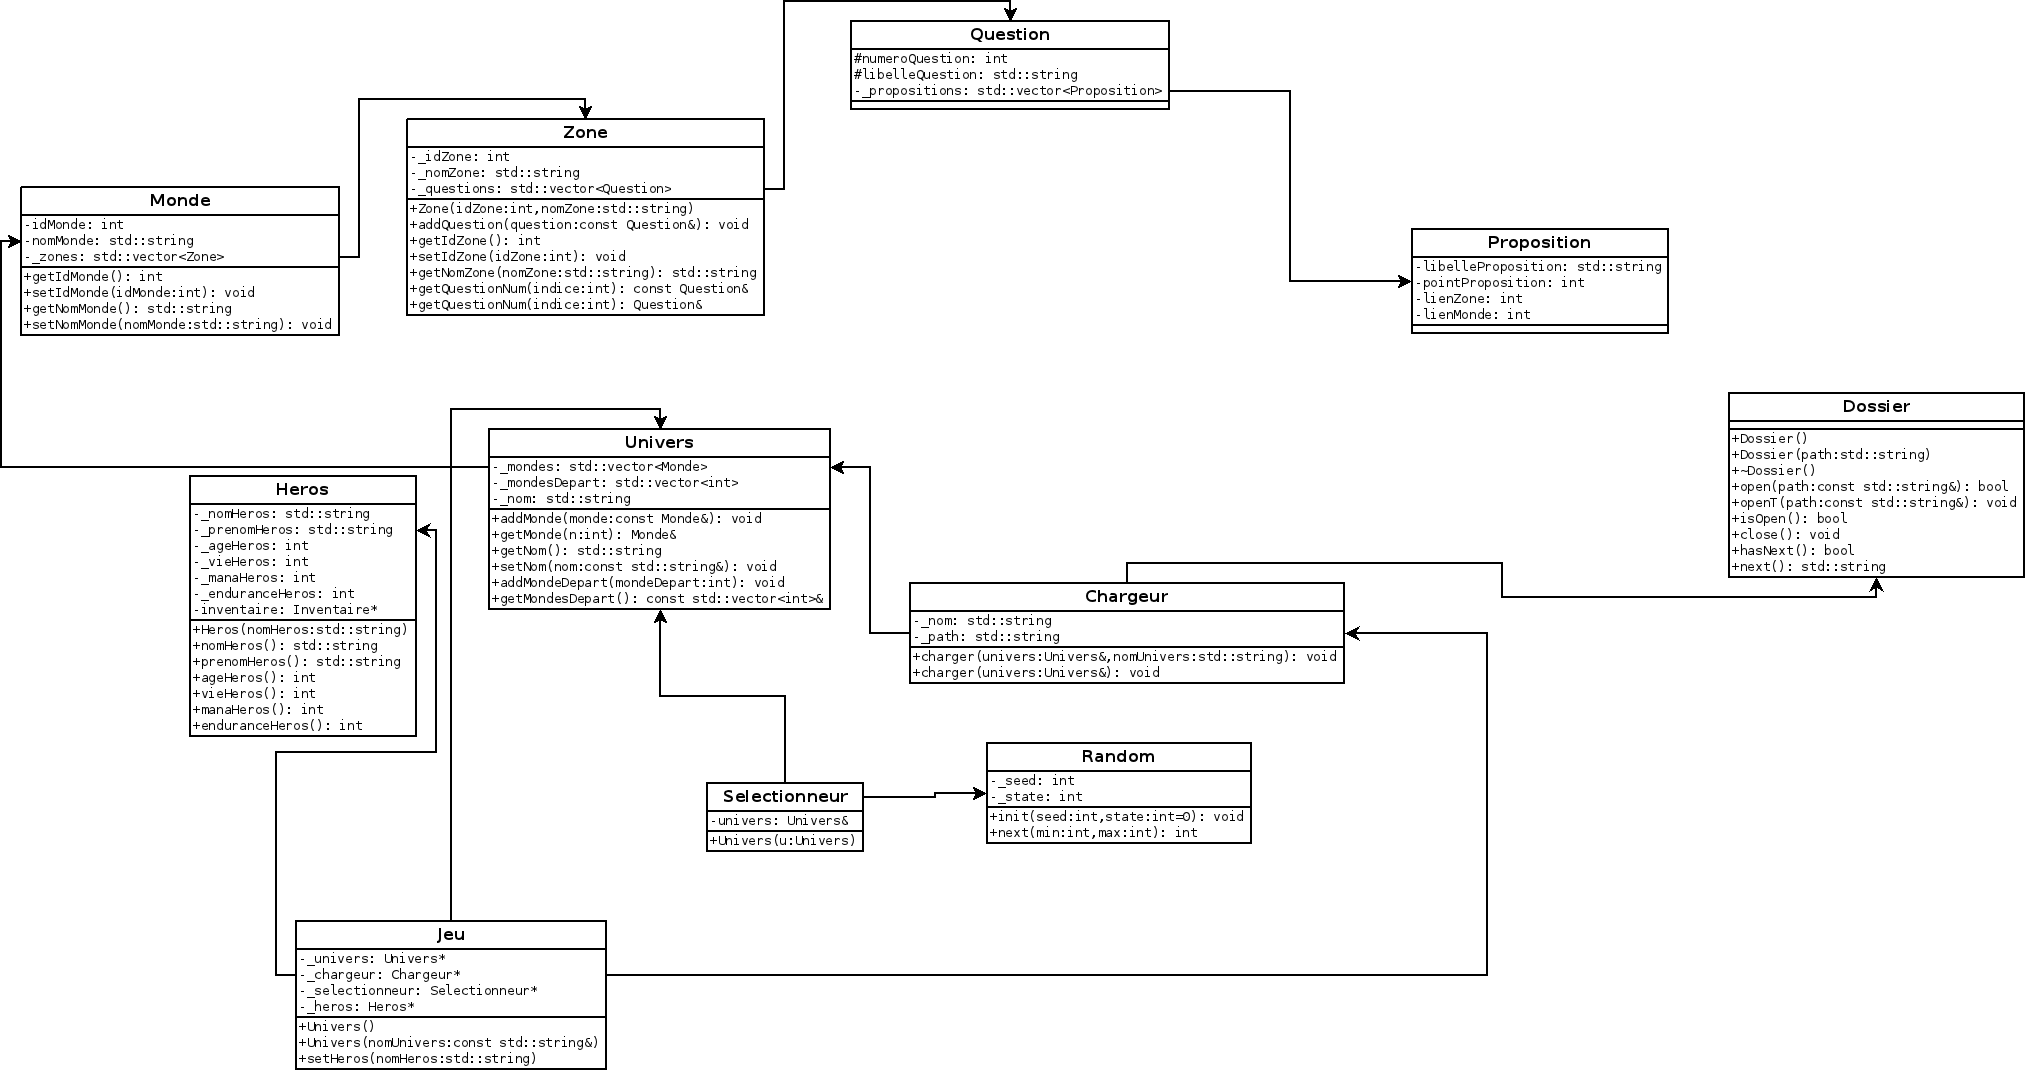
\includegraphics[scale=0.25]{figures/UML.png}
\caption{Partie du diagramme de classe de l'application}
\label{Partie du diagramme de classe de l'application}
\end{figure}